\startchapter{A suite of packages for scalable Whole Cell Models: WCMpy}
\label{WCMpy_chapter}

\section{Introduction}
The development of whole-cell models (WCMs) \cite{Bhat2020Whole-CellSurvey} is purported to be a defining challenge of the 21st century \cite{Tomita2001Whole-cellCentury}. WCMs amalgamate specialized models of cellular systems -- e.g. the metabolome and its kinetics rate laws; the genome and its translational units; and the proteome and its functional proteins -- into a single model that represents the entirety of a cell. This endeavor offers the unique opportunity to assess the completeness of cellular theory \cite{Palsson2000TheBiology,Feig2019Whole-cellDetail} and to answer research questions in medicine \cite{Bordbar2015PersonalizedPharmacodynamics,Loscalzo2011SystemsMedicine} and synthetic biology \cite{Purcell2013TowardsBiology}. WCMs are rooted in the Newtonian perspective that a complete model of both cellular biochemistry and environmental conditions can reproducibly recreate the phenotypes and diversity that are observed experimentally. An atomic-resolution molecular dynamics (MD) simulation of an entire cell (all $1E9$ molecules \cite[][approximated from cellular mass]{Lewis2014MassPopulations}) may be the ultimate tool to answer these audacious biological questions; however, since the state-of-the-art of MD is currently at the level of proteins \cite{Adcock2006MolecularProteins}, membranes \cite{Egberts1994MolecularMembrane,Alper1993ComputerDynamics,Alper1993TheStudy}, or small cells \cite{Perilla2015MolecularComplexes} for microseconds, WCMs are the state-of-the-art for simulating cellular chemistry \cite{Feig2015CompleteBiology} at biological timescales (hours to days). 

The first WCMs \cite{Karr2015TheModeling} were rudimentary systems of ordinary differential equations that often incorporated simplified assumptions of growth \cite{PERRET1960APopulation}, such as the Monod kinetics model \cite{Han1988ExtendedInhibition} which assumes that growth is solely contingent upon the glucose concentration. The advent of genome sequencing at the turn of the 21st-century \cite{Collins2003TheBiology, Covert2001MetabolicSilico} facilitated the development of genome-scale metabolic models (GEMs) \cite{Varma1994StoichiometricW3110,Edwards2000TheCapabilities}, which resolved genome-protein-reaction relationships \cite{Edwards2001InData} in metabolic systems and thereby improved the biochemical resolution of these WCMs from the original mathematical frameworks \cite{Gibson1988PredictingTemperature,Ho2021UnconventionalTargets}. 

GEMs are executed with the flux balance analysis (FBA) algorithm \cite{Orth2010, Lee2006FluxMetabolomics}, which distills metabolic systems into a matrix of reaction stoichiometry (S) and a vector (v) of variable reaction fluxes $\left( \frac{mmol}{g_{DW}*hour} \right)$. The S matrix consists of a row for each chemical, a column for each reaction, and the corresponding stoichiometry of a chemical in a reaction (negative for reactants, and $0$ for chemicals that are not in the reaction) as each matrix element. The S matrix for this example three reaction system
\begin{equation} \label{reactions}
    \begin{split}
        aA + bB &\xrightarrow{v_1} cC + dD \\
        aA + dD &\xleftrightarrow{v_2} yY + zZ \\ 
        cC + zZ &\xrightarrow{v_3} growth~,
    \end{split}
\end{equation}
would be $ 
    \begin{bmatrix} 
    -a & -a & 0 \\
    -b & 0 & 0 \\
    c & 0 & -c \\
    d & -d & 0 \\
    0 & y & 0 \\
    0 & z & -z 
    \end{bmatrix}~.
$
The v vector, e.g. $\begin{bmatrix} v_1 \\ v_2 \\ v_3\end{bmatrix}$ for the reactions of \cref{reactions}, contains the combination of reaction fluxes that corresponds with an optimum value of a metabolic objective, which is conventionally cellular growth ($growth$ in \cref{reactions}). Multiple different v vectors can correspond to the same optimized objective value, which defines a linear space of objectively equivalent flux vectors \cite{Nagrath2010SoftAnalysis} that is explored through a variation of FBA called flux variability analysis (FVA)  \cite{Gianchandani2010TheBiology, Gudmundsson2010ComputationallyAnalysis}. The FBA algorithm uses matrix algebra and a chemical steady-state for each metabolic concentration $\frac{dC}{dt}=S \cdot v=0$, where the biological objective of FBA is presumed to be $>10^{15}$ times slower than metabolic reactions per se \cite{Dantus1987Real-timeReactions}, to efficiently determine optimal v vectors. This feature allows FBA to execute without kinetic rate laws, which is essential since many metabolic reactions have not been kinetically described; however, FBA is consequently independent of time and is therefore not directly applicable in biological workflows such as WCMs that attempt to simulate biology over time. 

The dynamic FBA (dFBA) method introduces time dependency to the FBA algorithm through kinetic flux constraints. Mathematical constraints are boundaries -- e.g. $1$ and $5$ in this expression $1<x<5$ -- that in the context of FBA tighten the vector space, i.e. reduce the set of v vectors that yield the same optimization value \cite{Covert2008IntegratingColi}, to improve the accuracy and precision of flux predictions. Standard flux constraints are $[0,1000]$ for irreversible reactions and $[-1000,1000]$ for reversible reactions. These constraints, which coarsely represent metabolic limitations of substrate diffusion and thermodynamic favorability \cite{Peres2017HowModes}, approximately capture experimental systems \cite{Edwards2001InData, Kauffman2003AdvancesAnalysis}; nevertheless, constraints for other chemical influences \cite{Fleming2010IntegratedMetabolism}, such as the following few examples, improve the precision of FBA predictions \cite{Magnusdottir2017GenerationMicrobiota}: 
\begin{enumerate}
    \item \textbf{Physicochemical} - constraints that directly reflect physical laws of mass and energy conservation, and the thermodynamic favorability or free energy of a reaction \cite{Henry2007}
    \item \textbf{Topological} - constraints that reflect compartmentalization and chemical gradients within a cell \cite{Price2004Genome-scaleConstraints}
    \item \textbf{Environmental} - constraints that reflect nutritional limitations in the extracellular space 
    \item \textbf{Regulatory} - constraints that reflect feedback mechanisms which govern enzymatic activity \cite{Covert2001RegulationMetabolism}
\end{enumerate}
The kinetic constraints of dFBA constrain a reaction flux to known rate law for a reaction in the model \cite{Machado2012ExploringMetabolism, Pernice2019IntegratingPractice, Mahadevan2002DynamicColi,Mahadevan2003TheModels} -- e.g. $12.2\le v_1 \le 12.2$ for a calculated reaction flux of $12.2$. The dFBA method entails a few steps: 1) known rate laws, e.g. 
\begin{equation} \label{rate_laws}
    \begin{split}
        \frac{d[C]}{c*dt} = \frac{d[D]}{d*dt} = v_1 &= \frac{V_{max1}*[A]*[B]}{K_{M_1}*[A]+K_{M_2}*[B]} \\
        \frac{d[growth]}{dt} = v_3 &= \frac{V_{max3}*[C]*[Z]}{K_{M_5}*[C]+K_{M_6}*[Z]}
    \end{split}
\end{equation}
for the system of \cref{reactions}, calculate reaction fluxes based upon the chemical concentrations of the previous timestep ($[A]_{t-1}$, $[B]_{t-1}$, $[C]_{t-1}$, $[D]_{t-1}$, and $[Z]_{t-1}$), or the initial concentrations for the first timestep; 2) the FBA algorithm determines fluxes for reactions without a kinetic constraint; and 3) the present chemical concentrations ($[A]_t$, $[B]_t$, $[C]_t$, $[D]_t$, and $[Z]_t$) are updated with the sum of products of the chemical stoichiometry and the predicted fluxes of each reaction 
\begin{equation} \label{concentrations}
    \begin{split}
        [A]_t &= [A]_{t-1} +(- v_1*a - v_2*a)\\
        [B]_t &= [B]_{t-1} +(- v_1*b)\\
        [C]_t &= [C]_{t-1} + (v_1*c - v_3*c)\\
        [D]_t &= [D]_{t-1} + (v_1*d - v_2*d)\\
        [Z]_t &= [Z]_{t-1} + (v_2*z - v_3*z)\\
    \end{split}~~~.
\end{equation}
These steps repeat with each timestep. 

The ability to tailor constraints for a variety of chemical phenomena allows the FBA algorithm to studying numerous perturbations of metabolism. A few noteworthy applications of FBA include: e.g. medicine, through a) understanding diseases \cite{Chowdhury2020LeveragingApplications}, b) studying bacterial growth rate \cite{Kauffman2003AdvancesAnalysis}, c) predicting the lethality of gene knockouts \cite{Covert2008IntegratingColi}, d) assessing the efficacy of antimicrobial agents \cite{Lee2006FluxMetabolomics}, and e) investigating microbial communities \cite{Zomorrodi2012OptCom:Communities, Khandelwal2013CommunityGrowth} such as the human microbiome \cite{Shoaie2015QuantifyingMicrobiome, Kumar2019ModellingMicrobiome}; bioengineering, through rationally designing a) cultured-meats \cite{Suthers2020ChallengesModeling}, b) nutritious crops \cite{Schwender2008MetabolicPlants, Allen2009MetabolicComplexity, Potrykus2001GoldenAward, Tang2009GoldenA}, and c) biofuel-producing microorganisms \cite{Pham2021Genome-scaleProduction}; and bioremediation, through elucidating the involvement of microbes \cite{Rubinstein2021ORTCodes}.

Other sub-cellular systems, besides the metabolome, are included in WCMs: notably, the genome and the proteome. The genome, for example, begets the proteome, which in turn contributes $\frac{1}{3}$ of cellular mass \cite{Vakser2019ComputationalCell} and governs the metabolome through enzymatic catalysis. The transcription and translation processes between the genome and proteome are collectively termed the Central Dogma of biology
\begin{equation} \label{central_dogma}
    \ce{DNA ->[transcription] RNA ->[translation] proteins}~.
\end{equation}
The Central Dogma can be specified in simple models to occur at experimentally-determined rates, while more intricate models of epigenetics, for example, may require more complex representations of the Central Dogma to ensure that homeostasis is maintained during a simulation \cite{Karr2012}.

\subsection{Biofilm models}
A novel and aspirational application of WCMs is to simulate entire colonies of bacteria. Bacterial colonies (biofilms)  \cite{Otto2018StaphylococcalBiofilms,Mazza2016TheIntroduction} are an interesting subject of study since they cause persistent infections \cite{Lebeaux2014Biofilm-RelatedAntibiotics,Metcalf2013BiofilmEvidence,Jamal2018BacterialInfections,Singhai2012AResistance,Coenye2007BiofilmFactors,Baldan2014AdaptationCo-infection,Kropec2005Poly-N-AcetylglucosamineInfection,Potera1999ForgingDisease,Ramsey2004PseudomonasEnvironments,Stewart2014BiophysicsInfection}, and degrade industrial surfaces \cite{Herzberg2007BiofoulingPressure,Herzberg2008PhysiologyAeruginosa,Matin2011BiofoulingPrevention}, such as boat hulls \cite{Schultz2011EconomicShip,1952ChapterFouling,Coetser2005BiofoulingSystems,Callow2002MarineProblem}. Biofilms are additionally resistant to antimicrobial agents \cite{Lewis2001RiddleResistance} as the consequence of a) inter-species cohabitation \cite{Pereira2011SusceptibilityStudy}, which diversifies cellular vulnerabilities; b) limited diffusion through the polymeric biofilm matrix \cite{Suci1994InvestigationBiofilms,Hoyle1992PseudomonasPiperacillin,LeChevallier1988InactivationBacteria,Dunne1993DiffusionBiofilm,DeBeer1994DirectDisinfection}, which hinders liquid-state antibiotic treatments; and c) lower metabolic activity \cite{Mah2001MechanismsAgents,Sauer2004CharacterizationBiofilm,Suntharalingam2005QuorumFormation}, which limits antibiotic absorption.

Models of biofilm systems are empirical approximations of the underlying biochemical processes processes\cite{Wang2010ReviewBiofilms,Lewandowski20114.15Treatment,Wanner1986AModel,Tiwari2001ModelingApplications,Tiwari1997BiofilmMedium}. The Rittmann model \cite{Suidan1987CriteriaTypes}, for example, simplified biofilm growth to one-dimension, ignored extracellular polymeric substances, and, like many early biological models \cite{Kim1989ApproximateExpression,Torres2008KineticAnode}, employed Monod kinetics to represent cytosolic chemistry. Improvements upon these early models \cite{Wanner1984CompetitionBiofilms,Gadani1993AModel} has manifested in more sophisticated algorithms for representing biofilm systems. Two prominent examples are the cellular-automaton (CA) algorithm, which simulates a spatial lattice and uses deterministic rules of biochemistry, and the individual-based growth model (IbM), which represents biofilms as ecosystems of individual cells in a contiguous space \cite{Kreft1998BacSimGrowth} and uses stochastic rules of biochemistry. Contemporary biofilm models \cite{Xavier2005Biofilm-controlStudy,DeJong2017MathematicalGrowth} -- e.g. the digital biofilm model \cite{Barai2016ModelingBehavior} and the Unified Multiple-Component Cellular Automaton model \cite{Laspidou2004EvaluatingModel}, amongst others \cite{Laspidou2014MaterialProperties,Laspidou2005FiniteBehavior} -- iteratively approach a mechanistic framework of biofilm biochemistry, which remains the frontier of biofilm models \cite{Laspidou2010Cellular-automataCons}.

The amalgamation of WCMs with models of extracellular processes \cite{Das1991AEquation,Frederick2011ACommunities,Characklis1981MicrobialAnalysis.,Waters2005QUORUMBacteria,Miller2001QuoremBacteria} would provide a mechanistic biofilm model with unparalleled biochemical resolution. This synergy would elucidate details -- e.g. effects of antibiotics \cite{Suidan1987CriteriaTypes} or reactive oxygen species \cite{Lewandowski1991ReactionBiofilms} -- that can accelerate experimental research to combat problematic biofilms. The remaining challenges to realize this conceptual synergy are two-fold: 1) the computational expense of simultaneously simulating $\approx 1E3$ complete WCMs, one for each simulated cell in the biofilm, is untenable for personal computers; and 2) the quantity of experimental data that is needed to thoroughly parameterize each variable of each process in each cellular and intercellular system is a formidable bioinformatics bottleneck, which requires assembling and organizing bulk amounts of experimental data and which is unfortunately exacerbated by limited programmatic access to biochemical databases. 

\subsection{WCMpy suite}
We, therefore, developed a suite of Python modules -- inspired by the modularity of the Edinburgh Genome Foundry suite of packages \cite{Codons2021TheFoundry} for synthetic biology -- that address each of the aforementioned challenges that impede applying WCMs in a biofilm model. 1) The first challenge of computational expense is addressed by condensing the WCM into its essence -- being the metabolome and the Central Dogma -- with lightweight Python modules: dFBApy and Codons, respectively. The Codons module is distinguished from the only Python module of the Central Dogma ("Dogma") by i) providing extended functionality -- e.g. generating and searching FASTA files in BLAST (Basic Local Alignment Search Tool), similar to other packages \cite{Gilpin2016PyPDB:Bank} -- and ii) providing more documentation and a more intuitive application programming interface (API) that facilitate its usage. The dFBApy module is distinguished from the only other dFBA module for Python ("dFBA") by being i) amenable with Windows OS, which greatly expands its accessibility \cite{StatistaMarket2021}; ii) lightweight for large-scale simulations; and iii) compatible with the other modules within our ecosystem. 2) The second challenge of bioinformatics processing is addressed through the BiGG\_SABIO module, which we developed to bootstrap programmatic access with the SABIO reaction kinetics (SABIO-RK) database \cite{Wittig2012} -- the most curated source of biochemical kinetics data, versus alternatives like the BRENDA database \cite{Chang2021} -- and then to refine the assembled data into a form that is directly amenable with the dFBApy package. 

The aforementioned scripts -- Codons, dFBApy, and BiGG\_SABIO -- are designed to be amalgamated into a Python WCM package, e.g. WCMpy, which would be to our knowledge the first attempt i) to assemble a WCM in Python (the most popular programming language \cite{TIOBE2022}) and ii) to simplify the WCM framework for community-level simulations, notwithstanding prior work in assessing biofilm antimicrobial efficacy via FBA \cite{Sigurdsson2012ABiofilm}. We believe that these lightweight and open-source packages offer unique resources for developers to crowd-source simpler and more accessible WCMs that can scale to multicellular studies, which is complementary to increasingly fundamental WCMs \cite{Maritan2022BuildingCell} elsewhere in the WCM community \cite{Goldberg2018EmergingMethods,Shepelin2020BenchmarkingMetabolism}. 

\section{Methods}
The logic and calculations for each of the aforementioned packages are separately detailed in the following sections.

\subsection{BiGG\_SABIO}

The BiGG\_SABIO Python module first loads a (JSON) GEM model with the syntax of the BiGG models repository (the standard repository for GEMs) \cite{King2016BiGGModels}. The module is organized into two distinct processes and functions. The first function \pyobject{scrape\_bigg\_xls} a) parses the loaded model to determine all of its reactions and their database annotations; b) systematically searches each database annotation of each reaction, in addition to the reaction/enzyme name, in the SABIO-RK database via a Selenium Firefox webdriver \cite{vandenBroucke2018PracticalScience,Nyamathulla2021APython} that navigates the webpage and retrieves data from iframes; c) downloads all of the search results in a local folder in the directory of the parameterized BiGG model; d) concatenates the complete set of XLS files, after the downloading has concluded, into a single CSV file; and e) scrapes and downloads the names and values for each rate law variable of the CSV file into a JSON file. These processes require an extensive amount of time; hence, this first function tracks its progress and can be stopped and resumed at any point. The second function of BiGG\_SABIO \pyobject{to\_fba} processes and refines the downloaded CSV and JSON content into a single JSON file that is amenable with dFBApy, which contains both the essential rate law information and the related provenance to ensure transparency and reproducibility of simulation parameters. 

\subsection{dFBApy}
The dFBApy package simulates dFBA of a BiGG-formatted GEM, as an API wrapper for the COBRApy (Constraint-Based Reaction Algorithm in Python) FBA module \cite{Schellenberger2011QuantitativeV2.0,Lloyd2018COBRAme:Expression}. The dFBApy module operates through a series of steps. 1) Simulation details are parameterized -- e.g. the total simulation time, the timestep value, a (XML) GEM, and a JSON file of kinetic data -- which can be sourced from BiGG\_SABIO or customized elsewhere. 2) The parsed parameters are substituted into the available rate laws. 3) The \pyobject{simulate} function cycles through \cref{rate_laws,concentrations} of the chemical system and updates a Pandas DataFrame \cite{McKinney2011Pandas:Statistics} of all chemical concentrations after each timestep. The conversion of fluxes into concentration changes necessitates the cellular dry mass and the cellular volume of the simulated organism, which we estimate to be $0.2 pg$ \cite{Loferer-Krobacher1998DeterminationAnalysis} and $1 fL$ \cite{Lewis2014MassPopulations} for bacteria, respectively, although these can be parameterized by the user. 4) Concentration changes are graphically visualized via MatPlotLib \cite{Hunter2007Matplotlib:Environment}, and data of the fluxes and concentrations can be exported with the figure to a local folder. 

\subsection{Codons}
The Codons Python module conducts simple manipulations and analyses of a genetic sequence and its corresponding proteins: notably transcription and translation of the Central Dogma. The modular functions of Codons first accept a genetic sequence as either a string or a FASTA-formatted file \cite{Lipman1985RapidSearches} (the standard format for genetic and protein sequences, where a sequence is preceded by a description line: e.g. 
\begin{lstlisting}[label = fasta_protein]
>Protein - 35_residues - 4796.5_amu
\end{lstlisting}
that is denoted by a leading "$>$"). The \pyobject{transcribe} function conducts transcription with a regular expression \cite{Thompson1968ProgrammingAlgorithm} that simply exchanges all thymines (T's) with uracils (U's), or visa versa. The \pyobject{translate} function conducts translation according to the investigator's specifications, which optionally includes translating a) all possibly proteins, b) the complementary sense strand, and c) all three possible reading frames. The function operates by 1) determining the location of start codons, which can be tailored by the investigator; 2) grouping nucleotides into sets of three (codons); 3) translating the codons into corresponding amino acids per the Standard Codons Table, which can be tailored by the investigator to accommodate species variability; and 4) terminate the protein when a stop codon is reached. The Codons module further supports searching genetic and protein sequences through the NCBI BLAST database \cite{Johnson2008NCBIInterface.,Price2019CuratedGenomes} via the "BioPython" module \cite{Cock2009Biopython:Bioinformatics}, which acquires and downloads information about the parameterized sequence, or its proteins, and therefore assists in identifying homologues, functionality, and pertinent literature. The Codons module can finally create and export FASTA files from any parameterized genetic or protein sequence into a local folder. 

\subsection{WCMpy}
The aforementioned Python modules, or their core logic, may be aggregated into a single module (WCMpy) that follows the workflow of Figure \ref{wcmpy_workflow}. The Central Dogma would be conducted via Codons and can be parameterized to occur at fixed rates of $70 \frac{nucleotides}{second}$ \cite{Dennis2009VaryingColi,Vogel1995EffectsColi} and $\left(\dfrac{5 \frac{amino~acids}{second}}{1.31 \frac{doublings}{hour}}\right)$ \cite{Young1976PolypeptideRate}, respectively, where the latter rate is a function of the doubling time of the simulated bacteria. Protein degradation can be calculated with half-life probabilities ($\% ~remaining = 100*\left(\dfrac{1}{2}\right)^{\frac{\text{time}}{\text{halflife}}}$) where protein half-lives are determined by the N-end rule \cite{Tobias1991TheBacteria} in which the N-terminus residue of a protein dictates its degradation rate as being either $2~minutes$ or $>10~hours$. Translation and transcription in WCMpy would furthermore be limited by the cytoplasmic concentrations of amino acids and nucleotides, which connects to the metabolic activity that would be calculated via dFBApy (an alternative approach of simulating metabolism, based in thermodynamics, is proposed in the Supporting Information). The input file of kinetics rate laws for dFBApy in this workflow would ideally be sourced from BiGG\_SABIO. The extracellular concentrations, e.g. Lysogeny broth (LB) \cite{LysogenyBroth} that is approximated as degraded casein protein \cite{Jolles1962AminoPara--casein} and yeast extract \cite{YeastSpread}, may be user-specified in addition to the presence of antibiotics. The cellular mass, volumetric growth, and ultimately binary fission \cite{Donachie1968RelationshipReplication} (which we would presume to occur at a fixed rate like other WCMs \cite{Karr2012}) would be dependent upon the cytoplasmic concentrations at the end of a timestep, after the biochemical processes have occurred. The high-dimensional simulation results may finally be best communicated through visualizations of the cell or biofilm that complement the molecular-level data from the underlying dFBApy and Codons packages. 

\begin{figure}
    \centering
    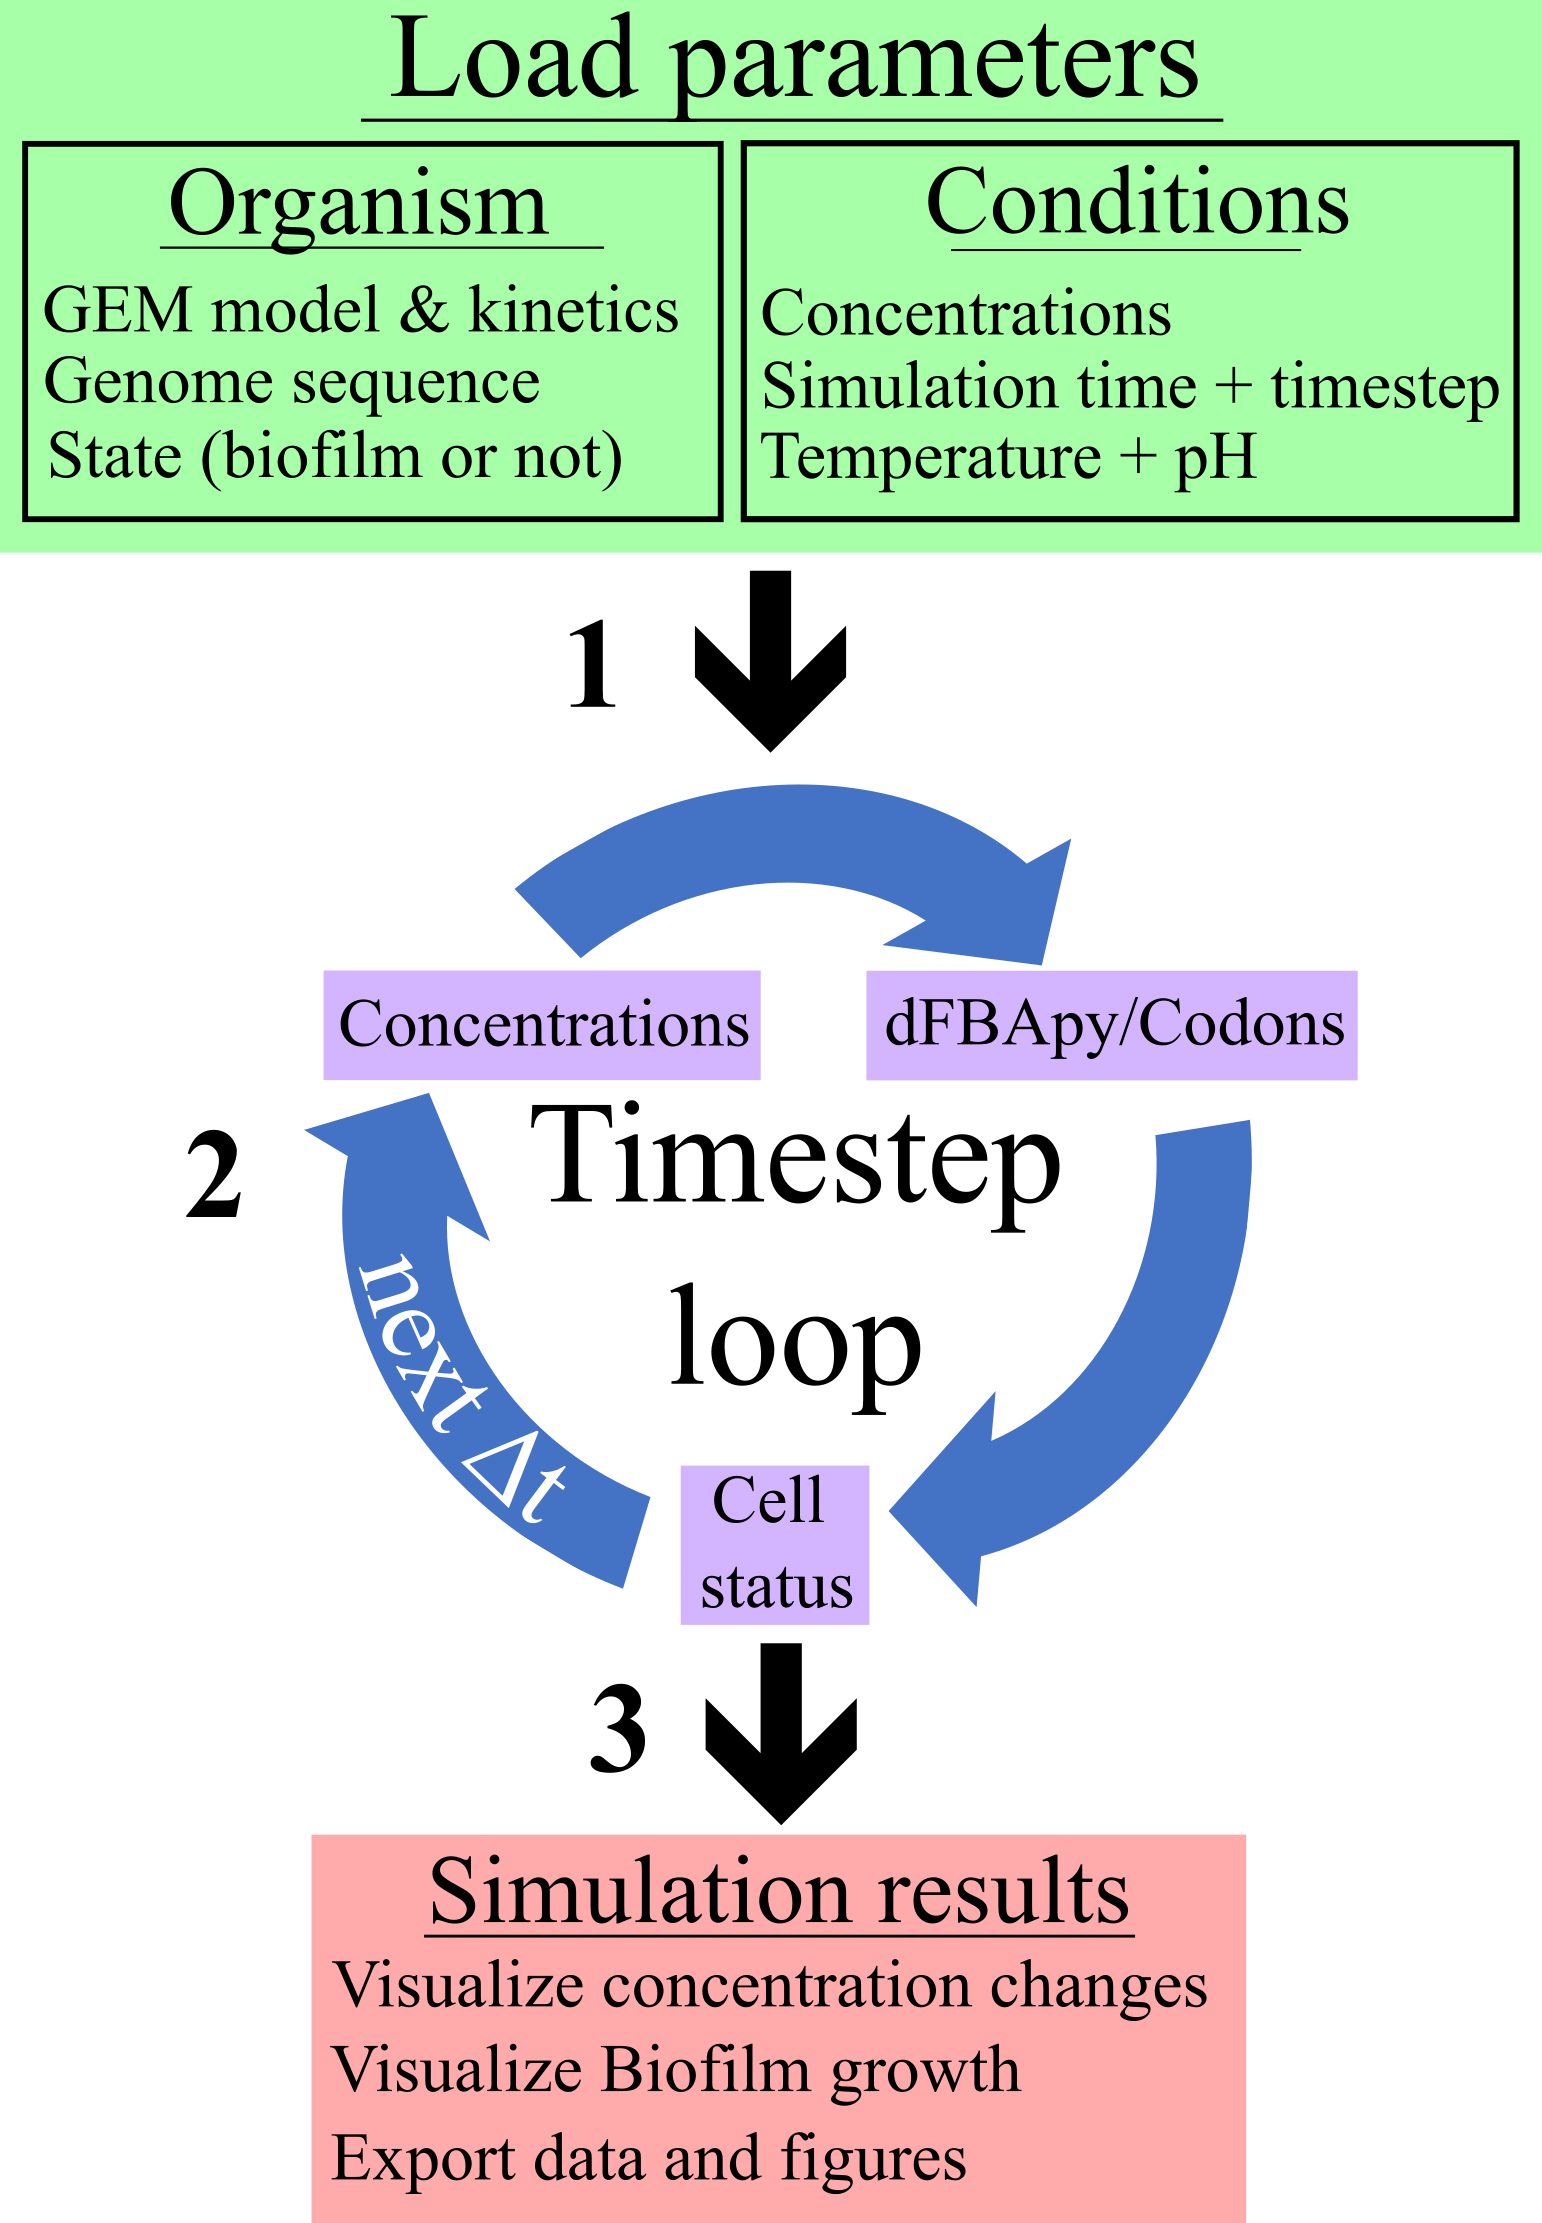
\includegraphics{images/WCMpy/wcmpy_workflow.png}
    \caption{
        The stepwise workflow of WCMpy. \textbf{Step 1} describes parameterizing the WCMpy simulation with information about the organism (e.g. the representative GEM and corresponding kinetics rate laws, the genome sequence, and the organismal state as either planktonic or sessile) and the simulation conditions (e.g. initial concentrations of the cytoplasm, the simulated time and timestep, and environmental conditions of the system). \textbf{Step 2} describes the loop that occurs with each timestep: a) dFBA and the Central Dogma are conducted based upon previous concentrations; b) the statuses of each cell and biofilm component are calculated; and c) the concentrations are updated by the reaction flux for the next timestep. \textbf{Step 3} describes processing, visualizing, and exporting the simulation results. 
    }
    \label{wcmpy_workflow}
\end{figure}

\section{Case studies}
We separately exemplify core functionality of the WCMpy workflow -- being the BiGG\_SABIO, dFBApy, and Codons modules -- in the following sections, which are available as Python Notebooks in the respective GitHub repositories.

\subsection{BiGG\_SABIO \& dFBApy}
The BiGG \textit{E. coli} core model consists only of the $95$ essential metabolic reactions for \textit{E. coli}. This model was first loaded into the BiGG\_SABIO module, where the \pyobject{parse\_data} function systematically acquired all of the data ($\approx 185 MB$) that describes the reactions of this model. The \pyobject{to\_fba} function then refined the raw data into a manageable file of kinetics data that was then directly parameterized into dFBApy and executed for an arbitrary amount of time. The results of this simulation are illustrated in Figure \ref{dfba}a, where the metabolic system re-establishes an equilibrium after the metabolism is perturbed by initial concentrations and rate law fluxes. The plotted concentrations for chemicals with defined initial concentrations are absolute concentrations, while those for chemicals without initial concentrations are only relative concentrations to the unknown initial concentration and are tagged with "(rel)" in the legend. The ability to alternatively parameterize kinetics data as an argument to the \pyobject{simulate} dFBApy function was demonstrated in Figure \ref{dfba}b by specifying only Acetate Kinase kinetic information from the full kinetic file of Figure \ref{dfba}a. 

\begin{figure}
    \centering
    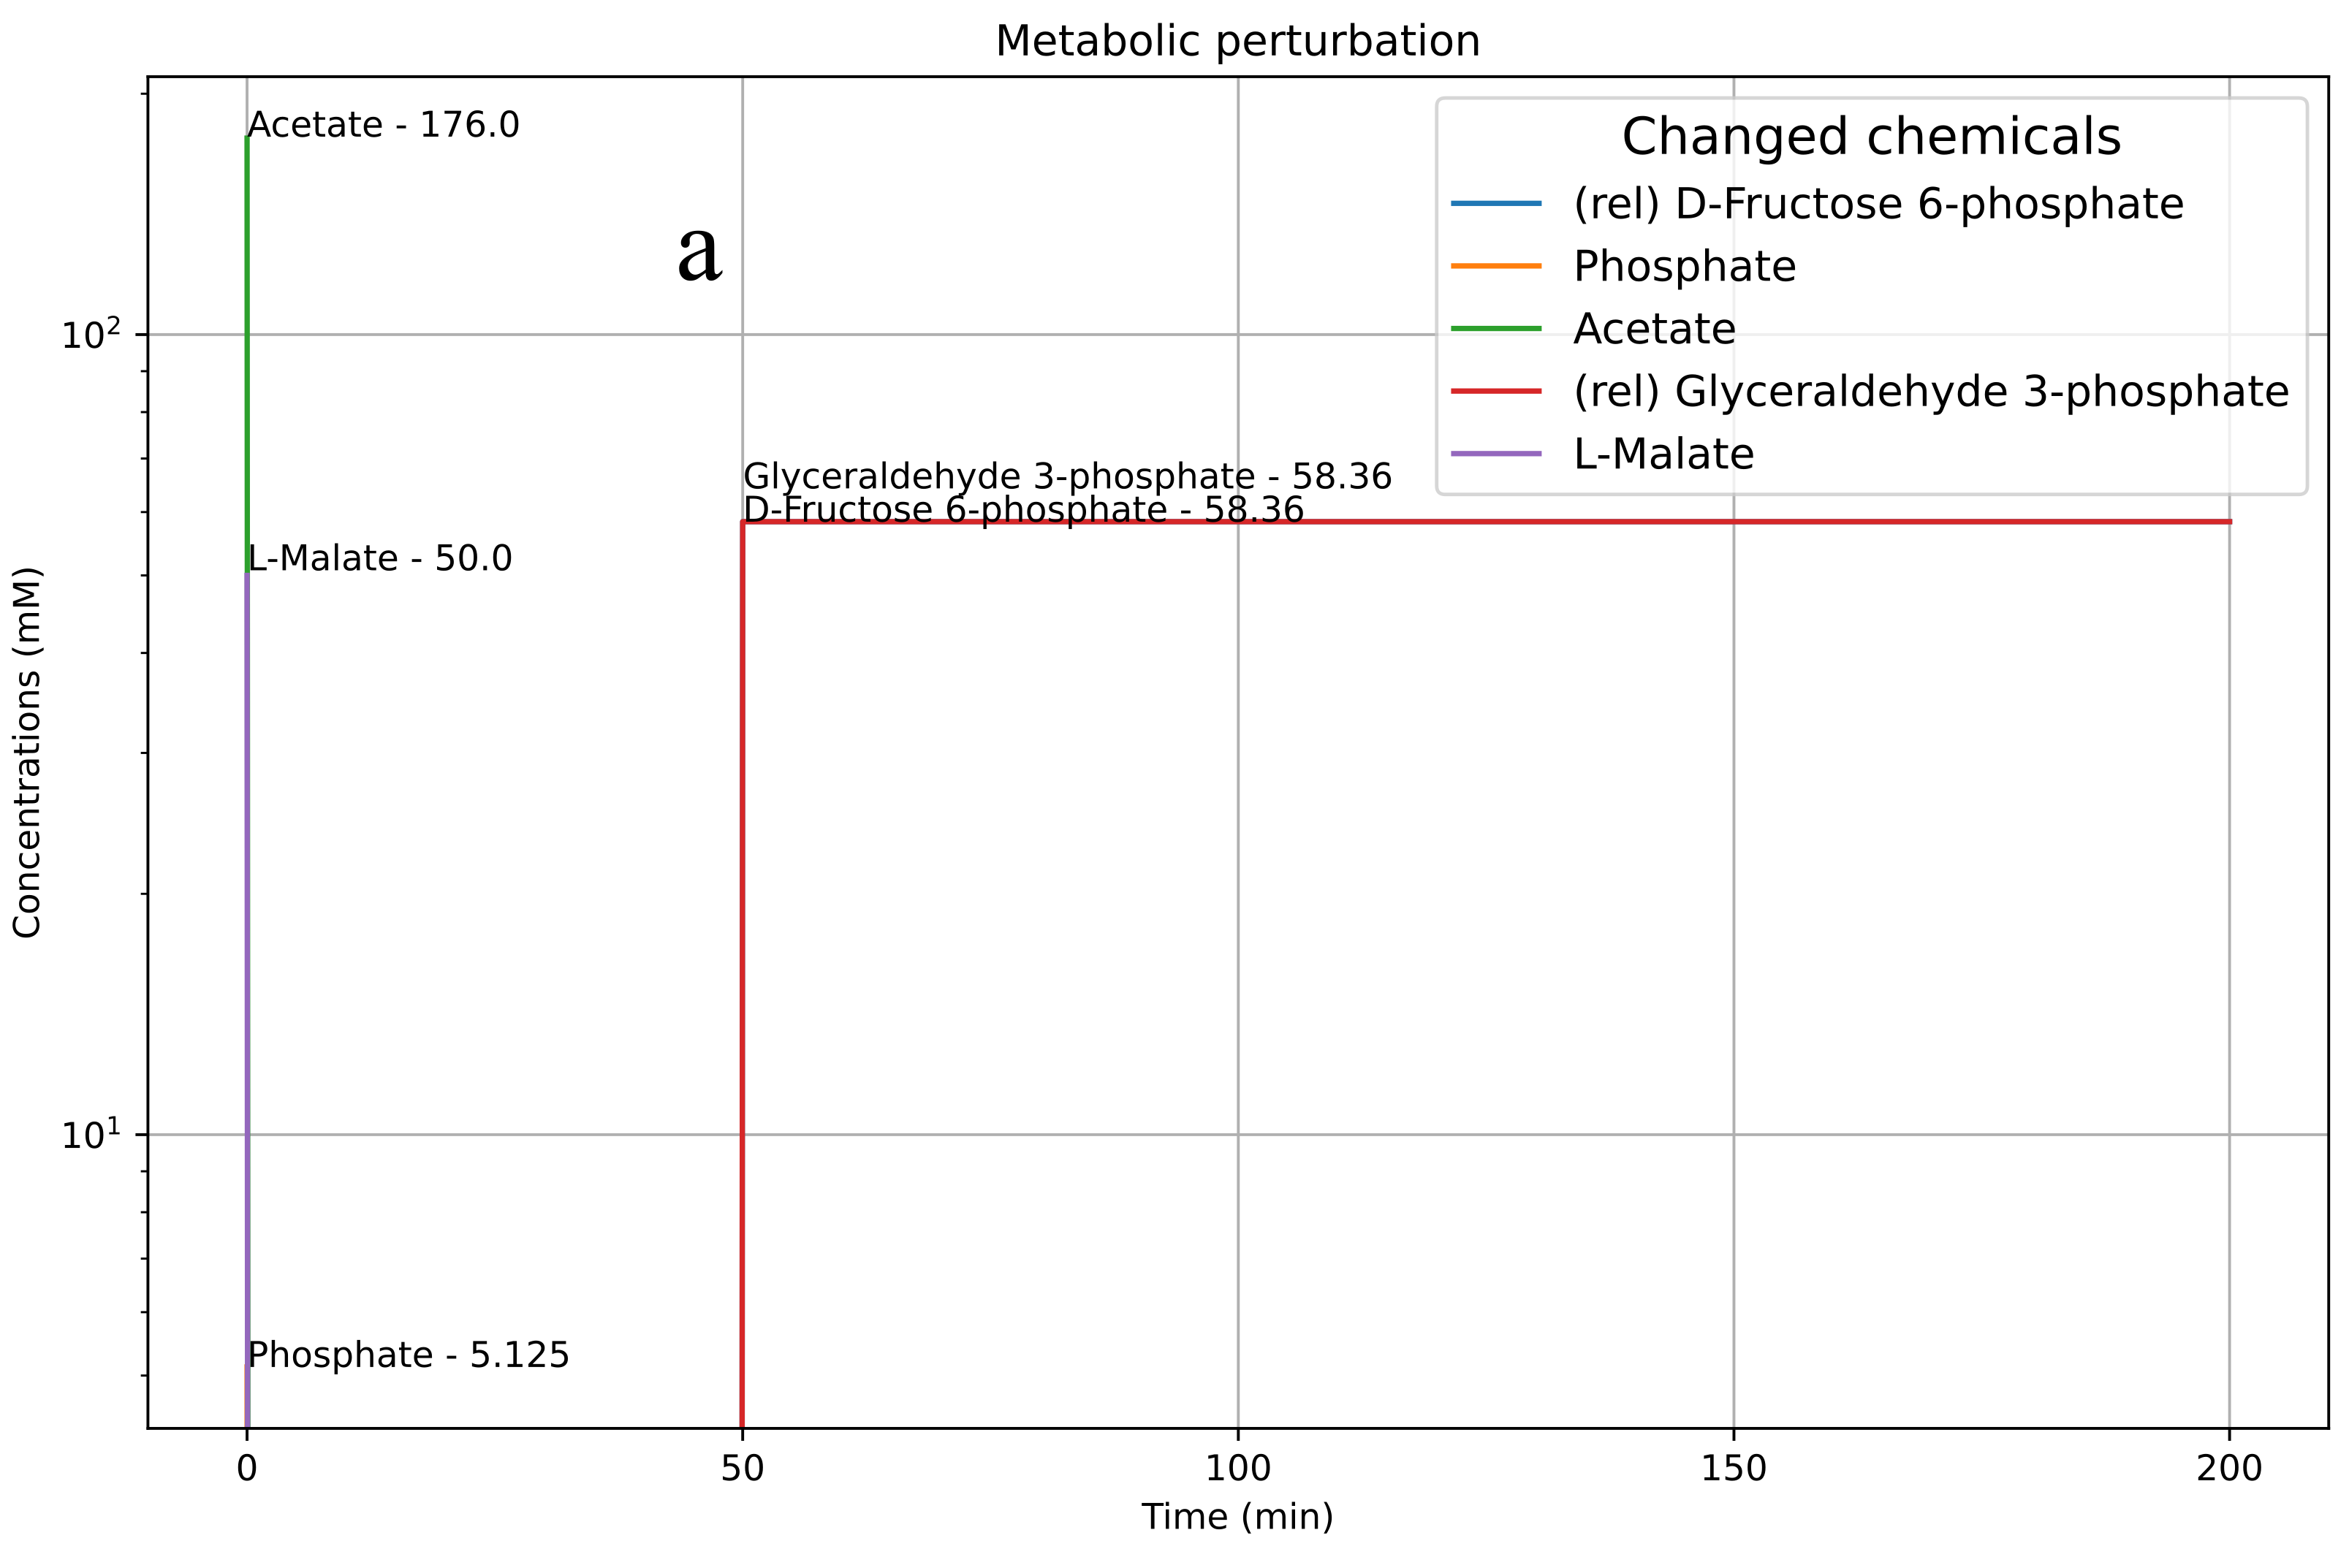
\includegraphics[width = 0.9\textwidth]{images/WCMpy/SABIO_dfba.png} \\
    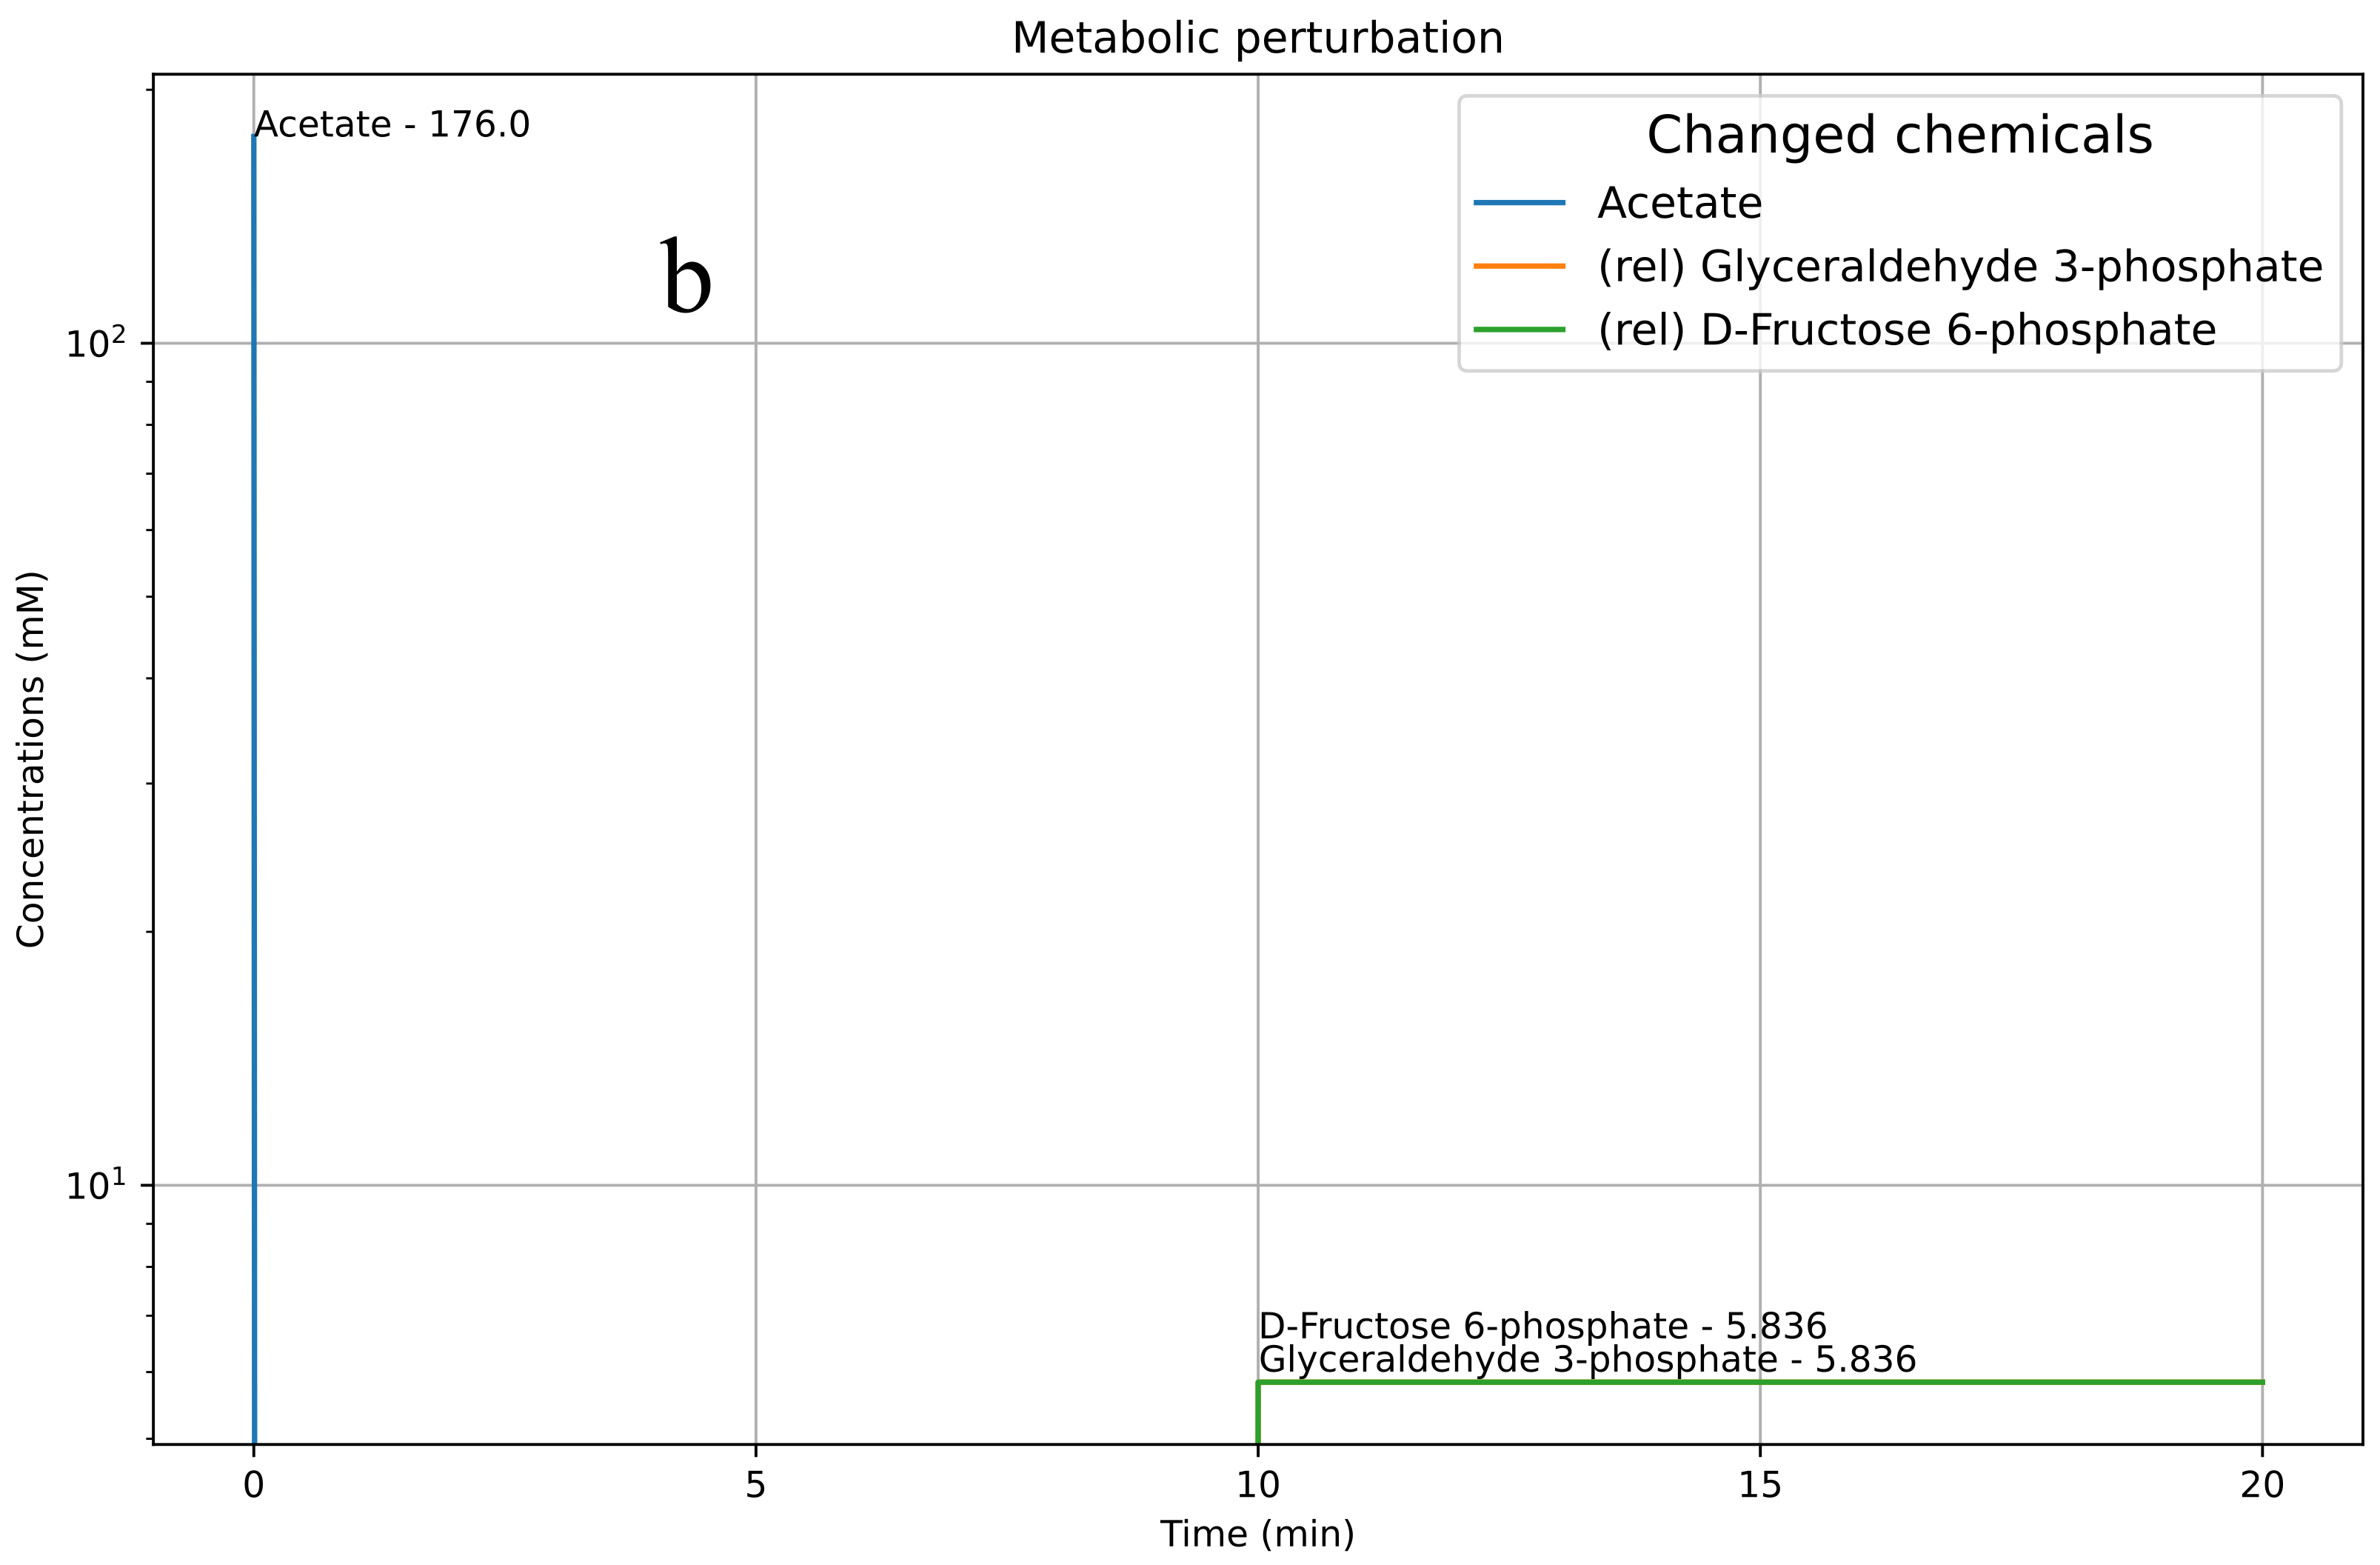
\includegraphics[width = 0.9\textwidth]{images/WCMpy/simple_argument.png}
    \caption{
        Notable concentration changes from simulating the \textit{E. coli} core BiGG model via dFBApy with a) full SABIO-RK kinetics data via the BiGG\_SABIO module and b) a single entry from the kinetics data that was passed as a function argument. Chemicals with defined initial concentrations are depicted at $t=0$, while other chemicals are labeled as relative changes "(rel)" since their initial concentrations are unknown. The metabolic consequences of these concentrations and calculated fluxes are observed over the first timestep, where equilibrium is re-established by generating D-Xylulose 5-phosphate and Alpha-D-Ribose 5 phosphate. The discrete establishment of equilibrium is the consequence of a "stiff" FBA algorithm. 
    }
    \label{dfba}
\end{figure}

\subsection{Codons}
The Central Dogma of the WC082 strain of Vancomycin-resistant \textit{S. aureus} \cite{Cong2020VancomycinFeatures}, sourced from the National Center of Biotechnology Information \cite{Haas2022StaphylococcusGenome}, was simulated through Codons. Between $[25,32]\%$ of the reported proteins, and $[65,83]\%$ of the reported peptide sequences, were perfectly translated from the 3 Mb genome -- depending upon which start codons were selected, how many open reading frames (ORFs) were translated, and whether the sense strand was translated. The translation of every possible protein, which accounts for overprinted genes, improved the accuracy to matching 41\% of proteins and 99.5\% of peptide sequences. Discrepancy between matches of entire proteins yet near 100\% matches of all peptide sequences supports that many bacterial proteins may be assembled from numerous peptides. Improvements in accuracy consequently increase a) the run time, from $1 min$ to $28 min$, and b) the proportion of false predictions, from 87\% to 97\%, for one ORF with no sense strand and for every possible protein on both strands, respectively. 

The aforementioned example with \textit{S. aureus} were contrasted with an example of the MERS (Middle-Eastern Respiratory Syndrome, $\approx 29kb$) virus \cite{Enouf2013MiddleGenome}. Slightly more of the reported proteins $\left(\frac{20}{30}\right)$ perfectly matched the translated proteins when considering all three ORFs, and 100\% of the reported proteins were perfectly translated when accounting for overprinted genes that are more common in viruses \cite{Ho2021UnconventionalTargets}, which suggests that viruses infrequently engage in peptide assembly into proteins. The sequences of the genome and the set of translated proteins were searched in the BLAST database through Codons, which were identified with 100\% certainty except for the small, ambiguous, peptides that are difficult to identify. 

\section{Discussion}
The developed suite of Python packages contributes modular tools that we postulate will foster the development of a mechanistic biofilm model, based upon a scalable WCM: WCMpy. The open-source Python community encourages collaboration, which may be particularly valuable for comprehensive projects such as WCMpy. The metabolome modules -- BiGG\_SABIO and dFBApy -- provide a conduit between a kinetics database and dFBA metabolic simulations for any organism whose metabolism is encapsulated in a BiGG-formatted GEM. These metabolic packages may individually useful to the DataNator \cite{Roth2021Datanator:Behavior} and ModelSEED \cite{Seaver2021TheMicrobes} WCM projects that are developing an improved bioinformatics resource and modelling tools, respectively. The dFBApy simulations are quantitatively consistent between the metabolic production in Figures \ref{dfba}a-b and the relative carbon input, which encourages their continued use by the community. The Codons module offers a rapid, intuitive, and practical tool for simulating the Central Dogma and investigating the genome and proteome of any organism with a known genetic sequence. These three packages advance available techniques to alleviate the noted bottlenecks -- scalable code and bioinformatics logistics -- that hinder developing mechanistic biofilm models with fundamental WCMs, which could expedite research in understanding and managing biofilms. 

\section{Author Contributions}
\begin{enumerate}
    \item \textbf{APF} - Writing and research
    \item \textbf{ESC} - Writing and research
    \item \textbf{HLB} - Writing, guidance, and funding
\end{enumerate}

\section{Acknowledgments}
The authors thank Jonathan R. Karr for his pioneering work in developing WCMs, and for providing guidance through our journey in systems biology.

% \setlength{\unitlength}{\savedunitlength}
